\newpage
\begin{appendices}
\iftoggle{commentboxes}{% Defined in packages.tex
	\gototoc
	\begin{tabular}{|p{\linewidth}|}
		\hline
		\begin{itemize}
			\item Add link to website for Excel file with tickers.
			\item Add reference to paper that compares YC from Bloomberg for the Euro area.
		\end{itemize}
		\\ \hline
	\end{tabular} \\}


	\begin{figure}[!htbp]
		\begin{centering}
			
			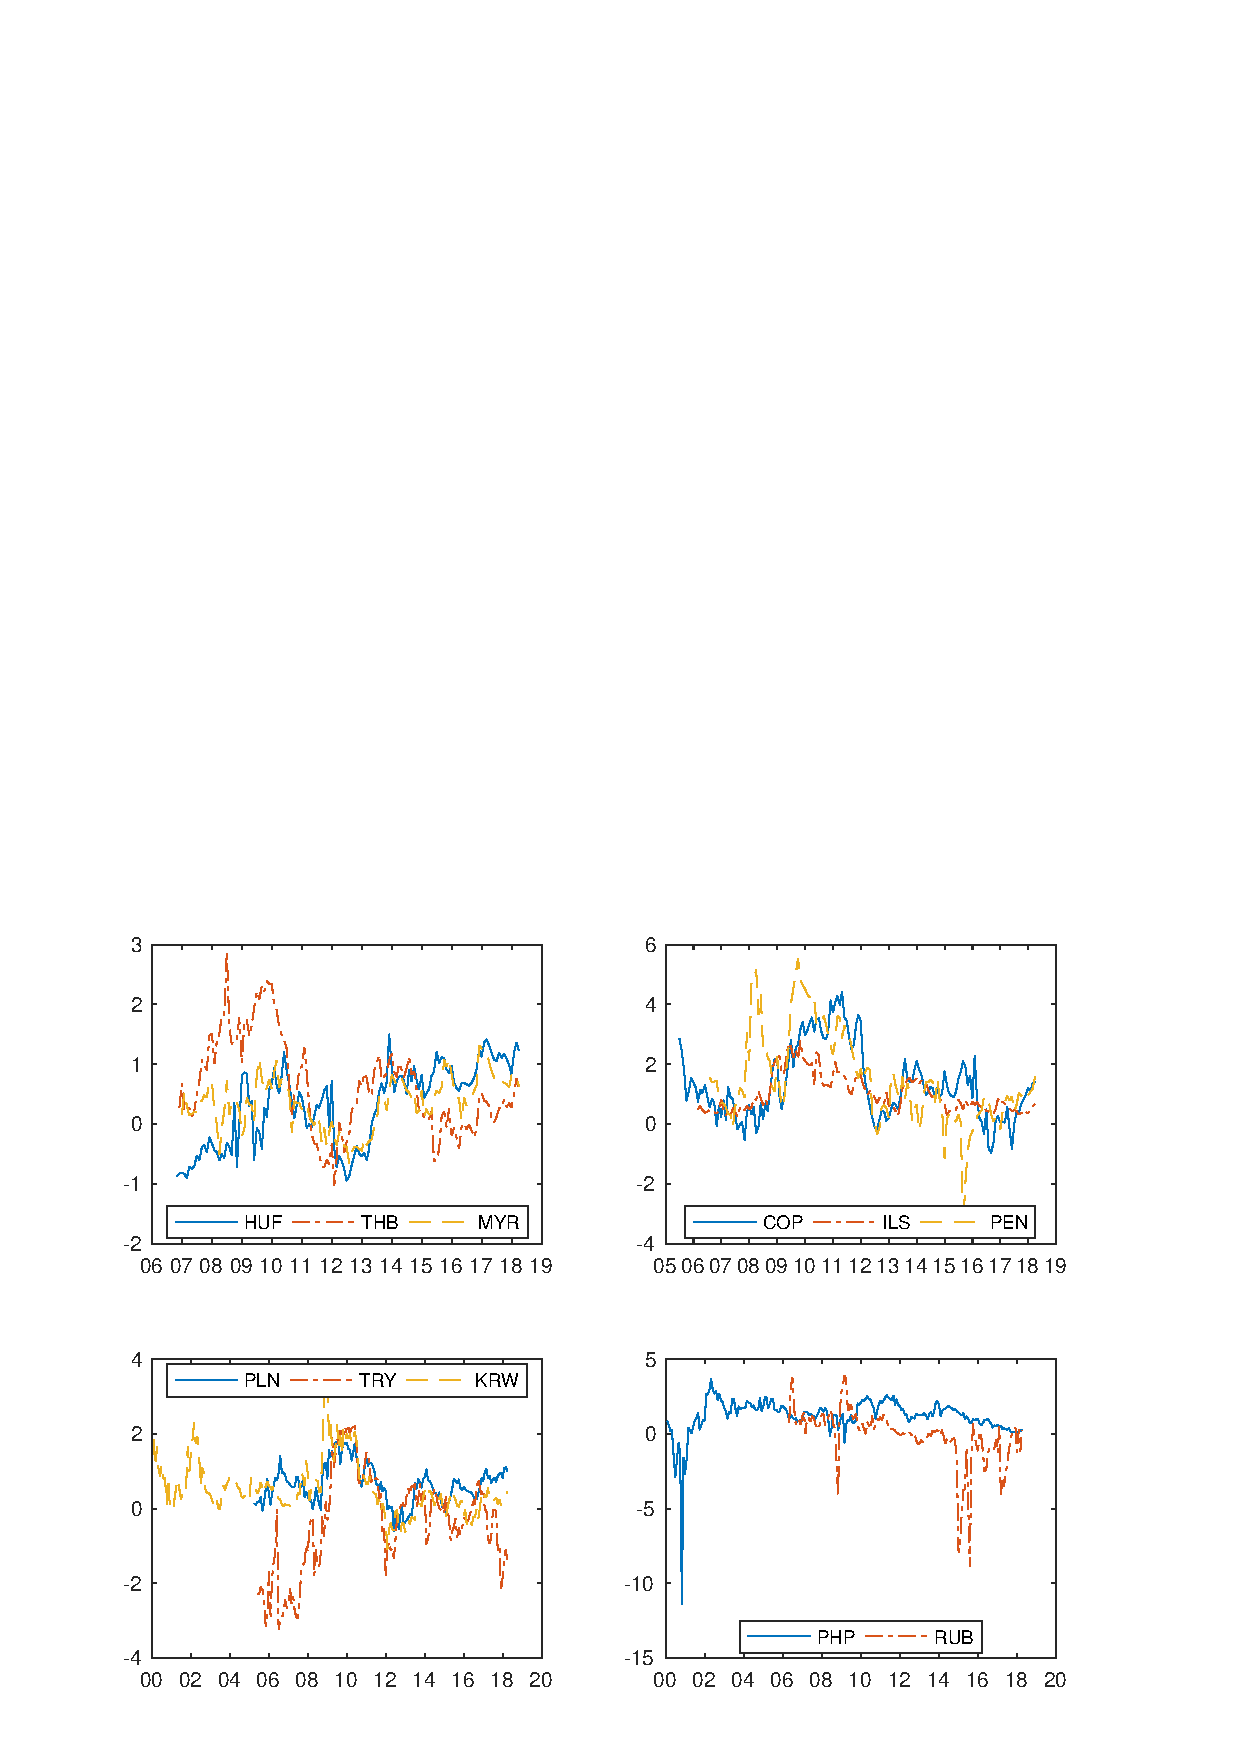
\includegraphics[width=0.9\textwidth,height=0.31\textheight]{../Figures/risk_premia_5yr_2}
			\newline

			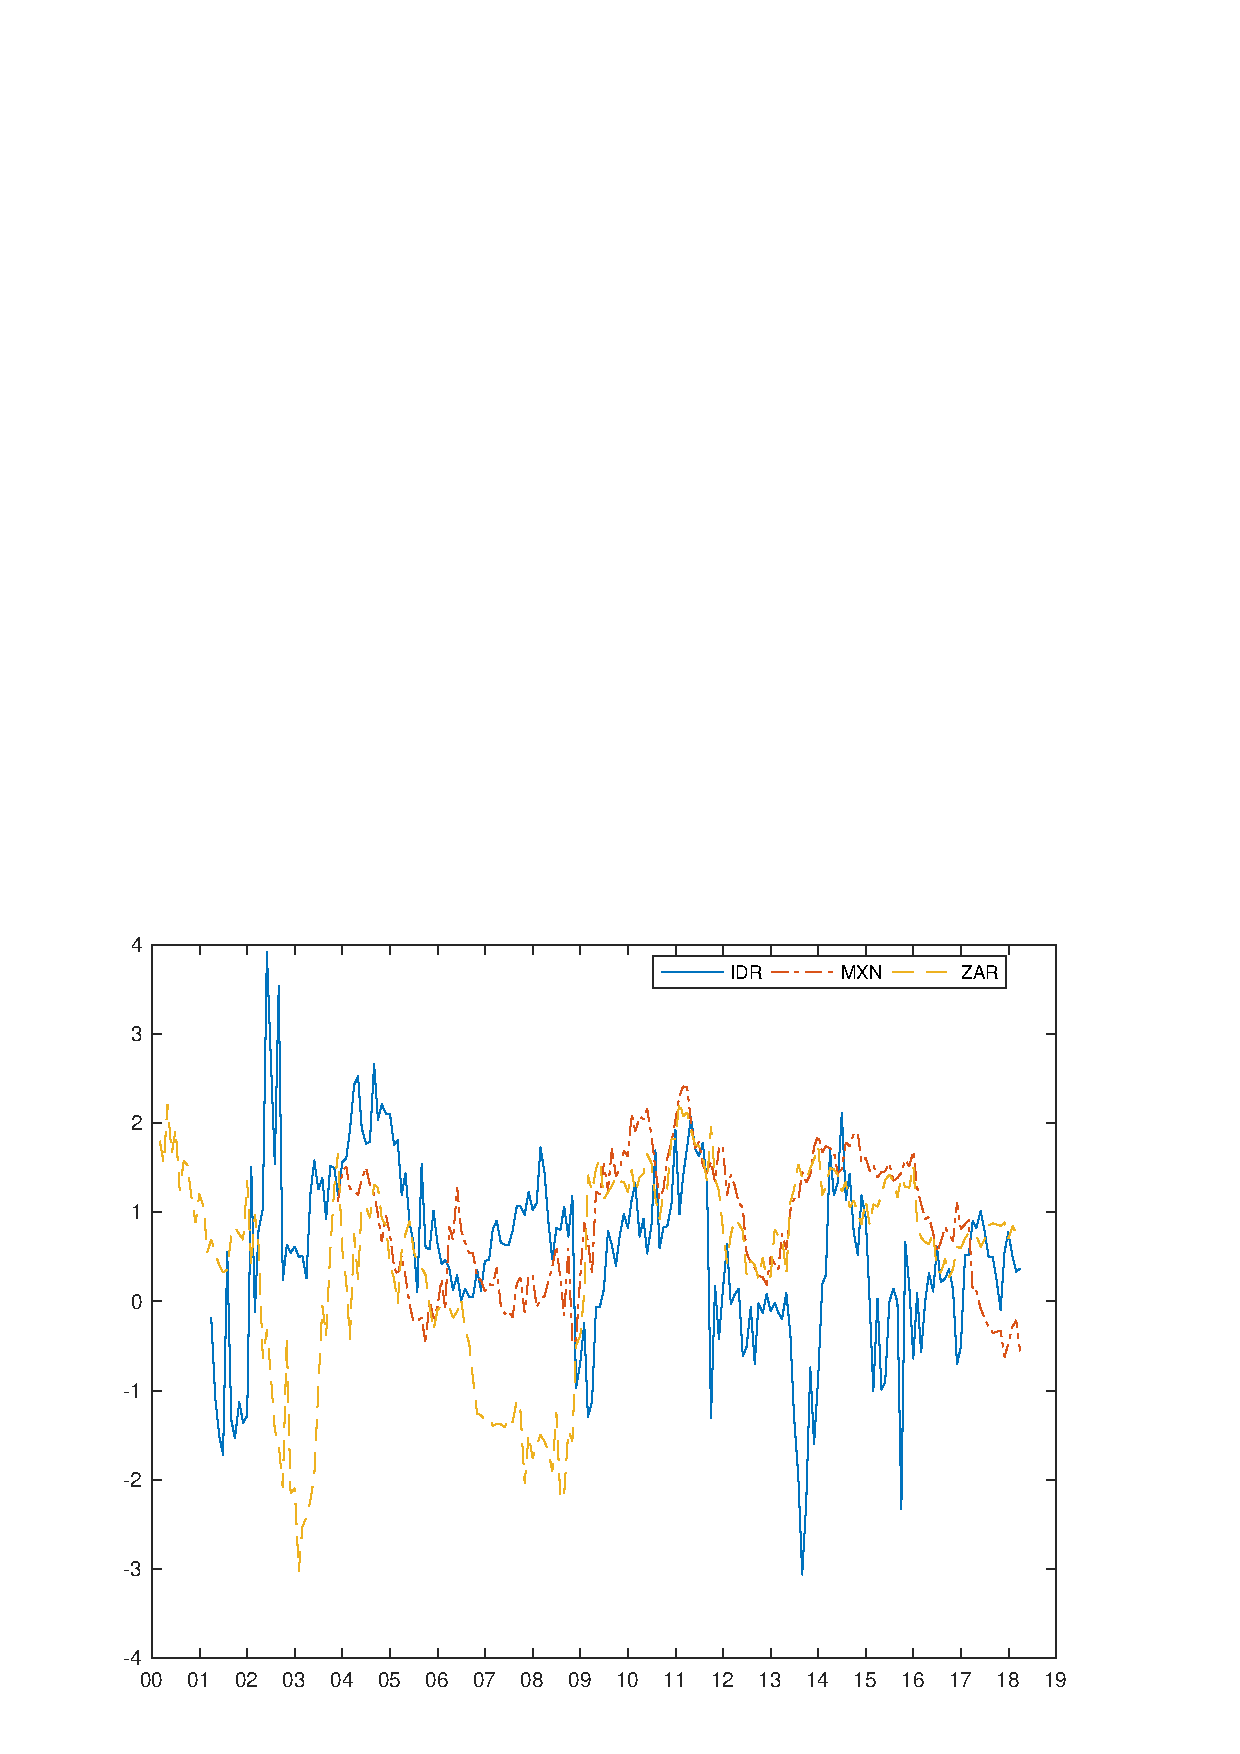
\includegraphics[width=0.92\textwidth,height=0.46\textheight]{../Figures/risk_premia_5yr_1}
			\par\end{centering}
		\caption{Estimated 5-Year Risk Premium.}\label{fig:5yr_rp}
	\end{figure}

\newgeometry{top=4cm, left=5.5cm}	% Modify this if more space is needed
%\newgeometry{margin=1cm}  % To make the table fit your landscape
\begin{landscape}

	\begin{table}
\centering
\begin{tabular}{l|cccccccccccccc}
\toprule
&\textbf{COP}&\textbf{HUF}&\textbf{IDR}&\textbf{ILS}&\textbf{MXN}&\textbf{PEN}&\textbf{PHP}&\textbf{PLN}&\textbf{TRY}&\textbf{KRW}&\textbf{MYR}&\textbf{RUB}&\textbf{THB}&\textbf{ZAR}\\\midrule
{ Coeff.}&1.17&-0.28&-0.32&1.02&0.42&1.50&-0.14&0.43&1.41&1.02&-0.23&1.37&0.82&-0.35\\\
{S.E.}&0.24&0.15&0.20&0.11&0.15&0.32&0.24&0.11&0.27&0.12&0.10&0.40&0.17&0.21\\\
{pVal}&0.00&0.07&0.10&0.00&0.01&0.00&0.55&0.00&0.00&0.00&0.02&0.00&0.00&0.10\\\
{Obs}&154&138&205&146&173&141&219&157&155&219&136&144&137&218\\\
{$R^2$}&0.13&0.02&0.01&0.37&0.04&0.13&0.00&0.10&0.16&0.26&0.04&0.08&0.15&0.01\\ \bottomrule
\end{tabular}
\\
\caption{Regression of 5-Year Risk Premium on $\ln (VIX)$.}\label{tab:rp_reg_lvix}
\end{table}
	
	\begin{table}
	\centering
\begin{tabular}{l|cccccccccccccc}
\toprule
&\textbf{COP}&\textbf{HUF}&\textbf{IDR}&\textbf{ILS}&\textbf{MXN}&\textbf{PEN}&\textbf{PHP}&\textbf{PLN}&\textbf{TRY}&\textbf{KRW}&\textbf{MYR}&\textbf{RUB}&\textbf{THB}&\textbf{ZAR}\\\midrule
{ Coeff.}&-0.21&-0.21&0.05&-0.16&-0.24&-0.02&-0.24&-0.02&-0.55&0.02&0.00&0.31&0.05&-0.18\\\
{S.E.}&0.05&0.03&0.04&0.03&0.03&0.08&0.04&0.02&0.04&0.02&0.02&0.09&0.04&0.04\\\
{pVal}&0.00&0.00&0.28&0.00&0.00&0.82&0.00&0.45&0.00&0.46&0.84&0.00&0.28&0.00\\\
{Obs}&154&138&205&146&173&141&219&157&155&219&136&144&137&218\\\
{$R^2$}&0.11&0.25&0.01&0.20&0.33&0.00&0.15&0.00&0.57&0.00&0.00&0.09&0.01&0.11\\ \bottomrule
\end{tabular}
\\
\caption{Regression of 5-Year Risk Premium on the Federal Funds Rate.}
\label{tab:rp_reg_ffr}
\end{table}
	
	\begin{table}
	\centering
\begin{tabular}{l|cccccccccccccc}
\toprule
&\textbf{COP}&\textbf{HUF}&\textbf{IDR}&\textbf{ILS}&\textbf{MXN}&\textbf{PEN}&\textbf{PHP}&\textbf{PLN}&\textbf{TRY}&\textbf{KRW}&\textbf{MYR}&\textbf{RUB}&\textbf{THB}&\textbf{ZAR}\\\midrule
{ Coeff.}&-0.00&0.02&-0.07&0.02&0.01&-0.18&-0.27&0.00&0.05&0.01&0.01&-0.08&0.01&0.02\\\
{S.E.}&0.02&0.01&0.02&0.02&0.02&0.08&0.04&0.01&0.03&0.02&0.02&0.03&0.04&0.02\\\
{pVal}&0.97&0.11&0.00&0.41&0.55&0.02&0.00&0.78&0.07&0.44&0.49&0.01&0.80&0.25\\\
{Obs}&153&137&204&145&172&140&218&156&154&218&135&143&136&217\\\
{$R^2$}&0.00&0.02&0.04&0.00&0.00&0.04&0.15&0.00&0.02&0.00&0.00&0.04&0.00&0.01\\ \bottomrule
\end{tabular}
\\
\caption{Regression of 5-Year Risk Premium on the Percentage Change of the Exchange Rate (LC per USD).}
\label{tab:rp_reg_rfx}
\end{table}
	
	\begin{table}
	\centering
\begin{tabular}{l|cccccccccccccc}
\toprule
&\textbf{COP}&\textbf{HUF}&\textbf{IDR}&\textbf{ILS}&\textbf{MXN}&\textbf{PEN}&\textbf{PHP}&\textbf{PLN}&\textbf{TRY}&\textbf{KRW}&\textbf{MYR}&\textbf{RUB}&\textbf{THB}&\textbf{ZAR}\\\midrule
{ Coeff.}&0.00&0.00&0.02&0.01&-0.00&0.00&-0.00&0.00&-0.00&-0.00&0.00&0.03&-0.01&0.04\\\
{S.E.}&0.02&0.01&0.01&0.01&0.01&0.02&0.02&0.01&0.01&0.01&0.01&0.02&0.01&0.02\\\
{pVal}&0.87&0.92&0.16&0.32&0.85&0.89&0.81&0.66&0.87&0.81&0.66&0.14&0.63&0.02\\\
{Obs}&153&137&204&145&172&140&218&156&154&218&135&143&136&217\\\
{$R^2$}&0.00&0.00&0.01&0.01&0.00&0.00&0.00&0.00&0.00&0.00&0.00&0.02&0.00&0.02\\ \bottomrule
\end{tabular}
\\
\caption{Regression of 5-Year Risk Premium on the Return of the Local Stock Market.}
\label{tab:rp_reg_stx}
\end{table}
	
	\begin{table}
	\centering
\begin{tabular}{l|cccccccccccccc}
\toprule
&\textbf{COP}&\textbf{HUF}&\textbf{IDR}&\textbf{ILS}&\textbf{MXN}&\textbf{PEN}&\textbf{PHP}&\textbf{PLN}&\textbf{TRY}&\textbf{KRW}&\textbf{MYR}&\textbf{RUB}&\textbf{THB}&\textbf{ZAR}\\\midrule
{ Inf.}&-0.30&-0.16&-0.08&0.21&-0.25&-0.73&NaN&0.05&-0.32&0.19&0.16&-0.10&0.07&-0.27\\\
{S.E.}&0.05&0.02&0.02&0.02&0.04&0.08&NaN&0.02&0.05&0.04&0.04&0.04&0.03&0.02\\\
{pVal}&0.00&0.00&0.00&0.00&0.00&0.00&NaN&0.04&0.00&0.00&0.00&0.02&0.02&0.00\\\
{Une.}&0.16&-0.05&0.29&NaN&0.62&0.83&0.32&NaN&0.40&0.35&0.81&0.95&0.98&NaN\\\
{S.E.}&0.06&0.02&0.04&NaN&0.05&0.09&0.04&NaN&0.06&0.13&0.17&0.14&0.18&NaN\\\
{pVal}&0.01&0.00&0.00&NaN&0.00&0.00&0.00&NaN&0.00&0.01&0.00&0.00&0.00&NaN\\\
{IP}&-0.01&0.00&NaN&-0.03&0.01&0.32&0.02&0.02&-0.01&0.01&NaN&-0.00&NaN&-0.05\\\
{S.E.}&0.02&0.00&NaN&0.01&0.01&0.05&0.00&0.03&0.01&0.01&NaN&0.03&NaN&0.01\\\
{pVal}&0.53&0.36&NaN&0.00&0.68&0.00&0.00&0.42&0.38&0.10&NaN&0.91&NaN&0.00\\\
{Obs}&154&138&205&146&159&124&159&157&155&219&98&144&137&218\\\
{$R^2$}&0.24&0.55&0.20&0.46&0.58&0.65&0.32&0.03&0.44&0.16&0.29&0.26&0.21&0.39\\ \bottomrule
\end{tabular}
\\
\caption{Regression of 5-Year Risk Premium on Macroeconomic Variables.}
\label{tab:rp_reg_macro}
\end{table}
	
\end{landscape}
\restoregeometry

\section{Nominal Yield Curve Construction} \label{sec:BFVcurves}
I use Bloomberg Fair Value (BFV) curves to estimate the nominal yield curve $\yLCnom$. BFV curves are par yield curves provided by Bloomberg on a daily basis for different maturities. These yields are converted into discount factors, which are then used to estimate the parameters in equation \ref{eq:NSSzero}. As with $\yLCsynt$, the parameters are chosen so as to minimize sum of squared deviations between the actual prices and the estimated prices weighted by the inverse of the duration of each security.

Not all maturities are available, that is why is important to obtained the implied zero-coupon yield curve.

I estimate curves from actual prices and they closely followed those reported by Bloomberg.

The tickers used to construct the nominal and the synthetic yield curves are provided in an Excel spreadsheet in the website.

\end{appendices}